% Changing book to article will make the footers match on each page,
% rather than alternate every other.
%
% Note that the article class does not have chapters.
\documentclass[letterpaper,10pt,twoside,twocolumn,openany]{book}

% Use babel or polyglossia to automatically redefine macros for terms
% Armor Class, Level, etc...
% Default output is in English; captions are located in lib/dndstring-captions.sty.
% If no captions exist for a language, English will be used.
%1. To load a language with babel:
%	\usepackage[<lang>]{babel}
%2. To load a language with polyglossia:
%	\usepackage{polyglossia}
%	\setdefaultlanguage{<lang>}
\usepackage[english]{babel}
%usepackage[italian]{babel}
% For further options (multilanguage documents, hypenations, language environments...)
% please refer to babel/polyglossia's documentation.

\usepackage[utf8]{inputenc}
\usepackage{hang}
\usepackage{lipsum}
\usepackage{listings}
\usepackage{hyperref}

\usepackage{dnd}

\lstset{%
  basicstyle=\ttfamily,
  language=[LaTeX]{TeX},
}

\usepackage{eso-pic}
\newcommand\BackgroundPic{%
	\put(0,0){%
		\parbox[b][\paperheight]{\paperwidth}{%
			\vfill
			\centering
			
\includegraphics[width=\paperwidth,height=\paperheight,%
			keepaspectratio]{img/paper.jpg}%
			\vfill
}}}

\title{Milton Manastorm, the Magnificient} 	
\author{Antonius Torode}
\date{Latest update: \today}


% Start document
\begin{document}

\AddToShipoutPicture*{\BackgroundPic}
\maketitle
\tableofcontents

% Your content goes here

% Comment this out if you're using the article class.
\chapter{Milton Manastorm Backstory}

Milton Manastorm comes from the Manastorm bloodline and is the twin brother to Millhouse Manastorm. Milton began studying Magic with his twin brother and continued to do so for years. They stuck together for most of their adventures. Of the two, Milton was the practival one who did the majority of work. He learned easier than Millhouse and was able to apply knowledge on a much more realistic level. On the otherwise, Millhouse was similarly just as powerful, but more interested in learning spells such as impending doom, with significantly unpractical cast times. Through their adventures, Milton was always saving his brother from the messes he would get into, secretly enjoying hte chaotic lifestyle they both lived.

Millhouse had a dream as a young boy to become a mage, a wizard. Milton had a similar dream, however he knew his brothers ego would not let them both do the same thing and thus Milton decided to become a sorcerer, allowing his brother to glory in his own self worth (as he saw wizards as the superior beings). As young boys they entered schools of magic, where they were both kicked out. Their mischief (especially when together) was more than the master sorceres and wizards could handle (mentally not physically). The skills and ability to learn magic for the twins was unrivaled. The bond of their bloodline gives them an increased interest and desire to constantly one up each other and enables them to pick up magic very simply.

Together, both the twins traveled all over hunting for rare and priceless artifacts. This was a sort of hobby for them. One day when trying to steal an ancient relic from a mysterious Naaru vessel, the two managed to find themselves split. Millhouse was sent to Arcatraz, a place of imprisonment for dangerous beings the Naaru encountered. He essentially became a stowaway who was in the wrong Naaru vessel at the wrong time. Milton on the other hand, who was similarly on that vessel, tried to escape from the encounter by casting plane shift. Unfortunately the Naaru, who were beings they knew virtually nothing about, caused some interrupting spell which cast Milton onto a far away plane, losing track of his brother. Since this point, they have been on separate paths.

When they were still young, the twins realized how much of a burden and flaw it was to rely on an arcane focus. Unfortunately they were unable to determine a way of not having to have one, but they did solve the flaw in having it be removable. Through a process the twins discovered while trapped (to be used as dinner) in an Orak camp, they found a way to embedd their arcane focus' as part of themselves.  The skin is cut with an Orak knife and pure molten gold is poured into the wound, which was a method the Orak used for tattooing the higher ranking members. Upon killing all members of the camp, they took the needed materials they looted, including the gold, and took it to an acquaintance they had traded a rare artifact to in Aurushire a few months back. This acquaintance was able to safely and very accurately perform this process. 

Milton had two different castings, one on the back of each hand. On the right hand, a hexagon gold cast was poured into his skin, a light red ruby lining with a white crystal in the center sealed in by the gold cast. On the left, a heptagon gold cast, with a dark violet ruby lining, and a black crystal in the center sealed in by the gold cast. On a prior expedition, when the twins were captured to be sacrificed in a village of dark monks, they took note of a balance the monks drew their power from. A balance of light and dark which gave these monks a harmony of power. After freeing themselves and destroying all of the monks, they acquired the most powerful stones from the leaders of the village. The white and black crystals are to represent the different sides of nature and the twins believed if they could harness their power in unison it would give them an enhanced balance of power. Since this time, they have been using the crystals as their arcane focus'.

As it stands, Milton is simply exploring the world, collecting rare and priceless artifacts, learning to increase his power/influence, and finding his brother. 

\chapter{Skills and Features}

\begin{paperbox}[float=!t]{Source of Power}
	The Manastorm bloodline has long been attuned with magic. The source of Milton's power comes from his magical bloodline. Unlike his brother Millhouse, Milton understands this. It does not give him a sense of weakness though. The strong background gives Milton the idea that he is able to do whatever it is he desires.
\end{paperbox}

\section{Class Features}

\subsection{Ability Scores (level 15)}
\stats[
STR = \stat{8},
DEX = \stat{12},
CON = \stat{18},
INT = \stat{16},
WIS = \stat{14},
CHA = \stat{20}
]

\subsection{Traits}
\begin{description}
	\item[Age:] 121
	\item[Alignment:] Chaotic Neutral
	\item[Size:] 2' 7"
	\item[Speed:] 25 ft.
	\item[Darkvision:] Dim light 60 ft as if lit.
	\item[Gnome Cunning:] You have advantage on all
	Intelligence, Wisdom, and Charisma saving throws
	against magic. 
	\item[Languages:] Common, Gnomish
	\item[Speak with Small Beasts:] Through sounds and
	gestures, you can communicate simple ideas with Small
	ar smaller beasts. Forest gnomes love animals and often
	keep squirrels, badgers, rabbits, moles, woodpeckers,
	and other creatures as beloved pets.
\end{description}

\subsection{Hit Points}

\begin{description}[font=\normalfont\textbf,noitemsep,topsep=1ex,leftmargin=1em]
	\item[Hit Dice:] 1d6 per level
	\item[Hit Points at First Level:] 6 + constitution modifier
	\item[Hit Points at Higher levels:] 1d6 (or 4) + constitution modifier per level 
\end{description}

\subsection{Proficiencies}

\begin{description}[font=\normalfont\textbf,noitemsep,topsep=1ex,leftmargin=1em]
	\item[Armor:] None
	\item[Weapons:] Daggers, darts, slings, quarterstaff's, light crossbows 
	\item[Tools:] None 
\end{description}

\begin{description}[font=\normalfont\textbf,noitemsep,topsep=1ex,leftmargin=1em]
	\item[Saving Throws:] Constitution, Charisma
	\item[Skills:] Arcana, Deception
\end{description}

\subsection{Equipment}

\begin{description}
	\item[Arcane Focus:] See backstory
	\item[Two Daggers:] Normal daggers, very sharp.
	\item[Stone of Good Luck:] While this polished agate is on your person, you gain a +1 bonus to Ability Checks and saving throws.
	\item[Gauntlets of Ogre Power:] Your Strength score is 19 while you wear these gauntlets. They have no effect on you if your Strength is already 19 or higher without them.
	\item[Cloak of Displacement:] While you wear this cloak, it projects an Illusion that makes you appear to be standing in a place near your actual location, causing any creature to have disadvantage on Attack rolls against you. If you take damage, the property ceases to function until the start of your next turn. This property is suppressed while you are Incapacitated, Restrained, or otherwise unable to move.
	\item[Bracers of Defense:] While wearing these bracers, you gain a +2 bonus to AC if you are wearing no armor and using no shield.
	\item[Quarterstaff:] An wooden staff with an embedded star ruby in the end. The wood is enchanted to be as hard as steel.
\end{description}

\subsection{Cantrips}

\begin{description}
	\item[Level 1:] Fire Bolt, Prestidigitation, Minor Illusion, Light, Mage Hand
	\item[Level 4:] True Strike
	\item[Level 10:] Shocking Grasp
\end{description}

\subsection{Spells}

\begin{description}
	\item[Level 1:] Magic Missile (1), Mage Armor (1)
	\item[Level 2:] Shield (1)
	\item[Level 3:] Scorching Ray (2)	 
	\item[Level 4:] Mirror Image (2)
	\item[Level 5:] Lightning Bolt (3)
	\item[Level 6:] Blink (3), Fireball (3)
	\item[Level 7:] Greater Invisibility (4)
	\item[Level 8:] Confusion (4)
	\item[Level 9:] 
	\item[Level 10:] Hold Monster (5)
	\item[Level 11:] Disintegrate (6)
	\item[Level 12:]
	\item[Level 13:] Finger of Death (7)
	\item[Level 14:] 
	\item[Level 15:] Dominate Monster (8)
\end{description}

\subsection{Spellcasting Ability}

\begin{description}
	\item[Spell save DC:] 8+proficiency bonus + charisma modifier
	\item[Spell attack modifier:] proficiency bonus + charisma modifier
\end{description}

\subsection{Flexible Casting}

\begin{description}
	\item[Creating Spell Slots: ] You can transform unexpended sorcery points into one spell slot as a bonus action on your turn.
\begin{dndtable}
	\textbf{Spell Slot Level}  & \textbf{Sorcery Point Cost} \\
	1st  & 2 \\
	2nd & 3 \\
	3rd & 5 \\
	4th & 6 \\
	5th & 7
\end{dndtable}
	\item[Converting a Spell Slot to Sorcery Points:] As a bonus action on your turn, you can expend one spell slot and gain a number of sorcery points equal to the slot's level.
\end{description}

\subsection{Metamagic}

\begin{description}
	\item[Quickened Spall:] When you cast a spell that has a casting time of 1 action, you can spend 2 sorcery points to change the casting time to 1 bonus action for this casting.
	\item[Empowered Spell:] When you roll damage for a spell, you can spend 1
	sorcery point to re-roll a number of the damage dice up to your Charisma modifier (minimum of one). You must use the new rolls. You can use Empowered Spell even if you have already used a different Metamagic option during the casting of the spell.
	\item[Heightened Spell:] When you cast a spell that forces a creature to make a saving throw to resist its effects, you can spend 3 sorcery points to give one target of the spell disadvantage on its first saving throw made against the spell.
\end{description}

\subsection{Phoenix Sorcery}

\begin{description}
	\item[Ignite:] As an action, you can magically ignite a flammable object you touch with your hand. 
	\item[Mantle of Flame:] As a bonus action, you magically wreathe yourself in swirling fire. For 1 minute, you gain the following benefits:
	
	\begin{enumerate}
		\item You shed bright light in a 30-foot radius and dim light for an additional 30 feet.
		\item Any creature takes fire damage equal to your Charisma modifier if it hits you with a melee attack from within 5 feet of you or if it touches you.
		\item Whenever you roll fire damage on your turn, the roll gains a bonus to equal to your Charisma modifier. 
	\end{enumerate}
	
	Once you use this feature, you can't use it again until you finish a long rest. 
	\item[Phoenix Spark:]  if you are reduced to 0 hit points, you can use your reaction instead be reduced to 1 hit point, and each creature within 10 feet of you takes fire damage equal to half your sorcerer level + your Charisma modifier.
	
	If you use this feature while under the effects of your Mantle of Flame, this feature instead deals fire damage equal to your sorcerer level + double your Charisma modifier, and your Mantle of Flame immediately ends. Once you use this feature, you can't use it again until you finish a long rest. 
	\item[Nourishing Fire:] When you expend a spell slot to cast a spell that includes a fire damage roll, you regain hit points equal to the slot's level + your Charisma modifier. 
\end{description}

\onecolumn
\section{Sorcerer Leveling Table}
\begin{center}
	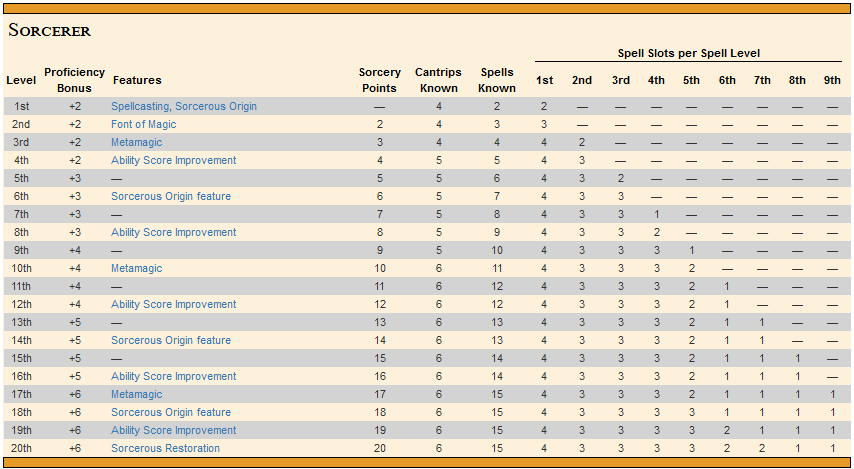
\includegraphics[width=\linewidth]{img/SpellSlotTable.png}
\end{center}




% End document
\end{document}
